\capitulo{3}{Conceptos teóricos}

\section{Conceptos teóricos básicos}

Para comprender este proyecto, es necesario familiarizarse con los siguientes conceptos teóricos básicos:
\begin{itemize}
    \item \textbf{Electroencefalografía}: Es una técnica de registro de la actividad eléctrica del cerebro. Se utiliza principalmente en medicina, psicología y neurociencia para estudiar el funcionamiento del cerebro.
    \item \textbf{Dispositivo Emotiv MN8}: Es un dispositivo de EEG portátil e inalámbrico que permite la recopilación de datos de EEG en tiempo real. Este dispositivo es capaz de registrar la actividad eléctrica del cerebro y transmitirla a una computadora o dispositivo móvil para su análisis. Se puede ver cómo es en la imagen \ref{fig: EmotivMN8} y también en que partes se colocan en la imagen \ref{fig: PosicionSensoresMN8}
    \begin{figure}[h]
    \centering
    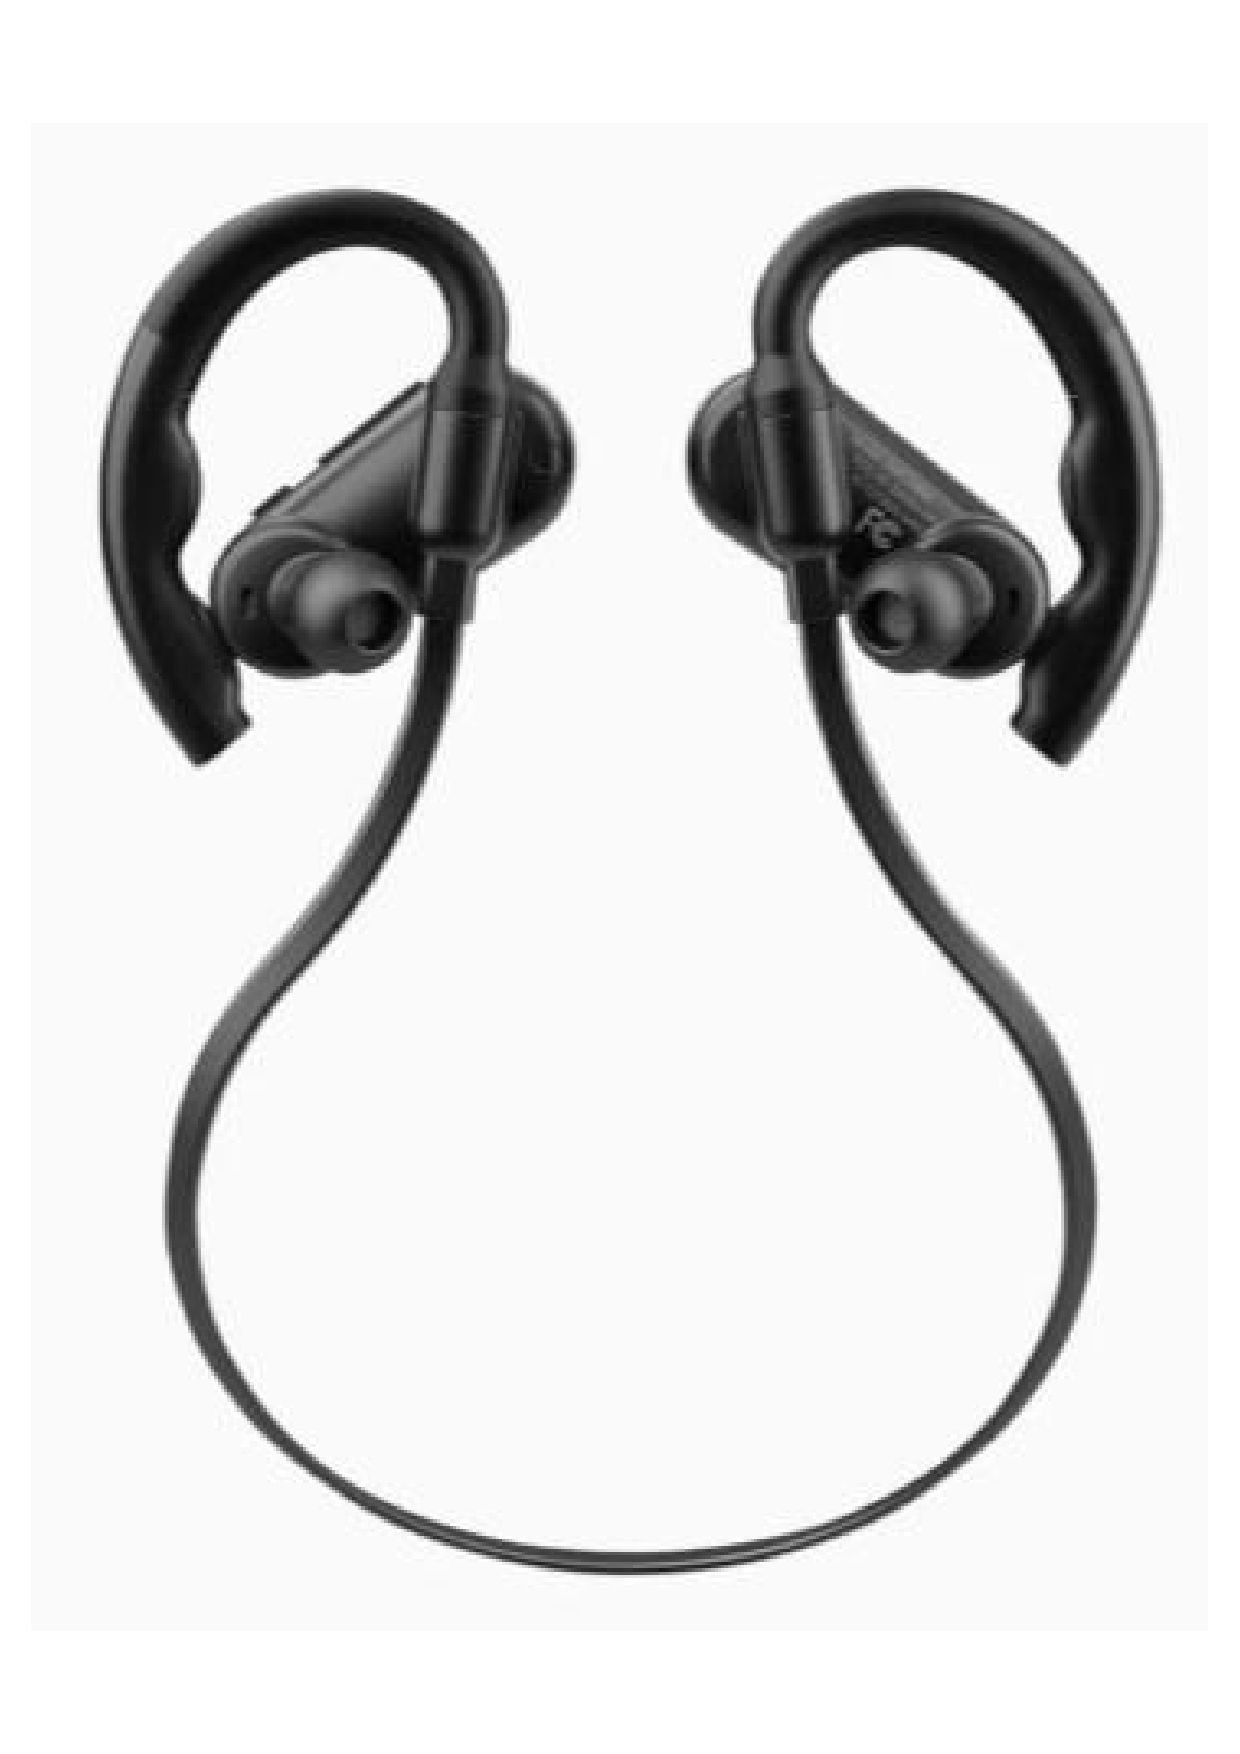
\includegraphics[width=0.3\textwidth]{img/DispositivoEmotivMN8.pdf}
    \caption{Dispositivo Emotiv MN8.}
    \label{fig: EmotivMN8}
    \end{figure}
    
    \begin{figure}[h]
    \centering
    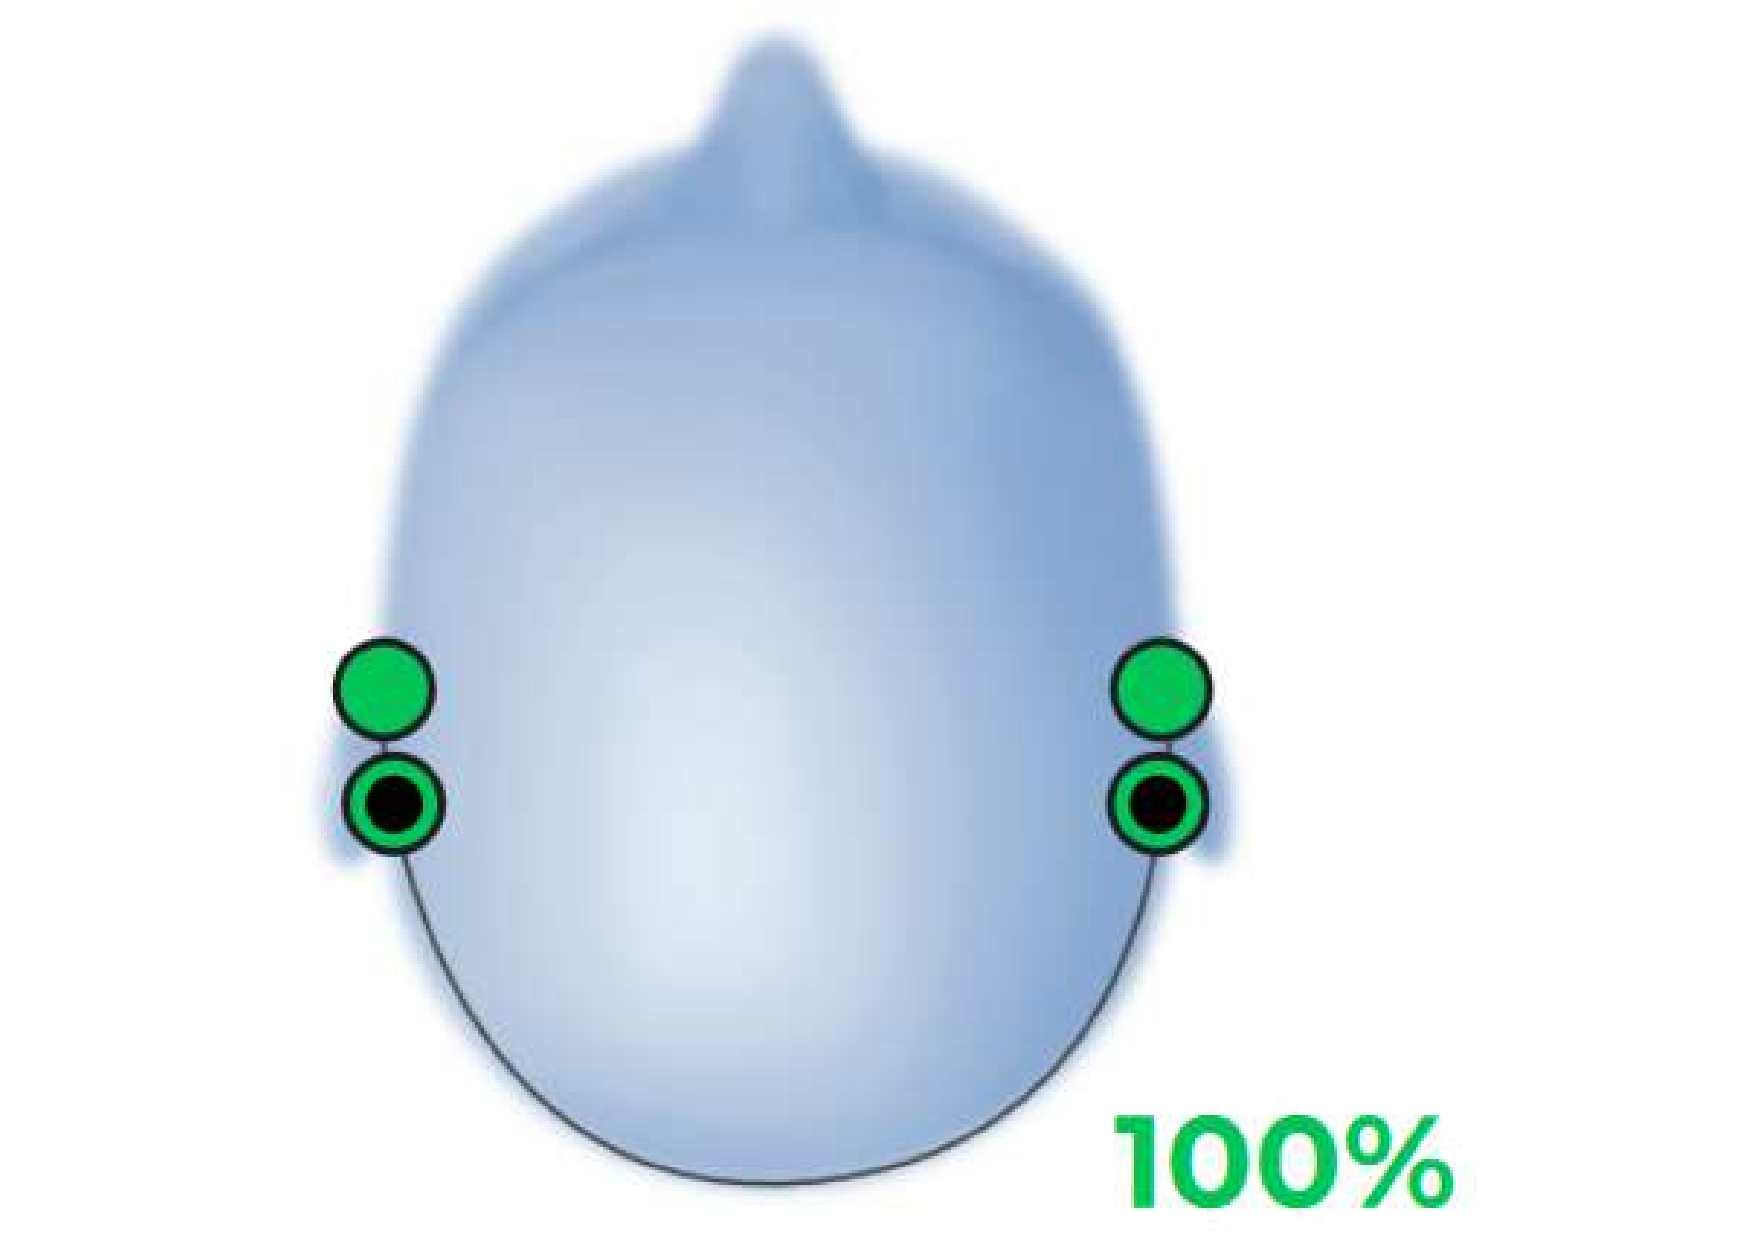
\includegraphics[width=0.5\textwidth]{img/PosicionSensoresMN8.pdf}
    \caption{Posición sensores MN8.}
    \label{fig: PosicionSensoresMN8}
    \end{figure}
    \item \textbf{Aplicaciones Emotiv y Contour}: Son aplicaciones de \textit{software} que se utilizan junto con el dispositivo Emotiv MN8 para recoger y analizar los datos de EEG. Estas aplicaciones permiten visualizar los datos de EEG en tiempo real y realizar análisis detallados de los mismos.
    \item \textbf{GitHub}: Es una plataforma en línea que facilita a las personas la posibilidad de trabajar en proyectos de programación de manera colaborativa. Permite a los usuarios guardar versiones de su código, lo que significa que pueden guardar diferentes versiones de su trabajo y volver a una versión anterior si es necesario. También proporciona un lugar para compartir proyectos de código abierto, lo que significa que cualquier persona puede ver, usar o contribuir a los proyectos alojados allí. Por lo tanto, es una herramienta útil para el desarrollo de software, ya sea de manera individual o en equipo. 
    \item \textbf{Diseño experimental}: Es el proceso de planificación de un experimento para asegurar que los datos recogidos sean válidos y confiables. En este proyecto, se diseñarán experimentos para crear situaciones controladas que permitan recoger y analizar los datos de EEG.
    \item \textbf{PsychoPy}: Es un \textit{software} gratuito que permite a los investigadores crear experimentos de neurociencia y psicología. Ofrece una interfaz sencilla para la presentación de estímulos y el control de experimentos, y puede ser utilizado tanto en ordenadores como en dispositivos móviles.
    \item \textbf{Análisis de datos}: Es el proceso de inspeccionar, limpiar y modelar los datos recogidos con el objetivo de descubrir información útil, informar conclusiones y apoyar la toma de decisiones.
    \item \textbf{Interfaz cerebro-computadora}: La interfaz cerebro-computadora, cuyas siglas son BCI y provienen de \textit{Brain–Computer Interfaces}, es un sistema que adquiere información neural, como datos de electrofisiología nerviosa o registros de ondas cerebrales, y la procesa e interpreta utilizando un ordenador \cite{InterfazBCI}\footnote{Artículo con información sobre qué es el BCI, así como su funcionamiento y sus aplicaciones \cite{InterfazBCI}.}. Estas interfaces permiten transformar el pensamiento en acciones reales en el entorno. Se aplican en diversas áreas, como la medicina (para el control de prótesis o rehabilitación), la investigación (con el estudio de la actividad cerebral) y la tecnología (por la interacción con dispositivos mediante el pensamiento).
    \item \textbf{EEG Headset}: Los \textit{EEG Headset} son dispositivos diseñados para medir y registrar la actividad eléctrica del cerebro. Estos dispositivos utilizan electrodos colocados en el cuero cabelludo para capturar los impulsos eléctricos generados por las células cerebrales o neuronas \cite{EEGHeadset}\footnote{Página web de Emotiv con toda la información general sobre los \textit{EEG Headsets} \cite{EEGHeadset}.}. Su uso se enfoca en comprender la actividad cerebral y su aplicación abarca desde la medicina hasta la investigación y la tecnología.
\end{itemize}
Estos conceptos proporcionan una base sólida para entender el proyecto y su objetivo de explorar el potencial de la tecnología EEG portable y su aplicación en el ámbito sanitario. Se espera que este proyecto proporcione una valiosa contribución a la comprensión de cómo se pueden utilizar los dispositivos EEG en la práctica médica y cómo los datos recogidos pueden ser utilizados para informar y mejorar las prácticas y estrategias.

\section{Estado del arte y trabajos relacionados.}
En esta sección, el conocimiento previo existente en el área específica del proyecto se analiza y se sintetiza en un resumen unificado. El propósito es situar el trabajo actual dentro del panorama científico y tecnológico, identificando las contribuciones previas, las limitaciones y las tendencias emergentes.
Por lo tanto, esta revisión abarca publicaciones científicas reales, patentes, proyectos previos y desarrollos relevantes.

\subsection{Aplicación de dispositivo de \textit{Interface neural} en Ingeniería de la Salud}
Para la realización de este proyecto, se ha tenido en cuenta el trabajo de fin de grado de Elena Pérez Barco, el cual es confidencial, por lo que no será referenciado para mantener la privacidad y derechos de autor, ya que el jurado tiene acceso a este trabajo.

Este trabajo se centra en una investigación comparativa de dispositivos EEG portátiles, analizando sus características técnicas, ventajas y desventajas, centrándose principalmente en el Emotiv Insight 2.0, un dispositivo EEG portátil ampliamente utilizado en investigaciones. Finalmente, se investigaron las posibles aplicaciones de estos dispositivos EEG portátiles en el ámbito de la salud.


\subsection{Dispositivos g.tec}
g.tec es una empresa que se encarga de desarrollar BCI y neurotecnologías de alto rendimiento, puediendo emplear técnicas invasivas y no invasivas en función del objetivo de las grabaciones \cite{g.tec}\footnote{Página web oficial de g.tec con información general de la empresa y sus productos \cite{g.tec}.}.

Uno de sus productos destacados es el g.Nautilus PRO, el cual se puede ver en la imagen \ref{fig: g.Nautilus}. Se trata de un auricular EEG portátil certificado por la CE (Conformidad Europea) y aprobado por la FDA (Administración de Alimentos y Medicamentos de los Estados Unidos) para registrar la actividad cerebral en entornos médicos y clínicos. Sus características más relevantes son \cite{g.Nautilus}\footnote{Sección del dispositivo g.Nautilus dentro de la página web oficial de g.tec \cite{g.Nautilus}.}:
\begin{itemize}
    \item Electrodos EEG: Disponible con 8, 16 o 32 electrodos EEG secos o húmedos prefijados para realizar un montaje más rápido.
    \item Versatilidad: Permite grabaciones secas y húmedas con un solo electrodo.
    \item Aplicaciones clínicas: Útil para monitoreo cerebral en entornos médicos y estudios de investigación.
    \item Electrodos activos: Hay 2 tipos de electrodos, electrodos activos secos 'g.SAHARA' o electrodos activos húmedos 'g.LADYbird'. Los electrodos 'g.SAHARA HYBRID' se caracterizan por:
    \begin{itemize}
        \item Tecnología patentada: Es el primer sistema de electrodos secos que funciona en todos los sitios cerebrales (frontal, central, occipital, temporal y parietal).
        \item Electrodo híbrido: Permite grabaciones secas y húmedas con un solo electrodo.
    \end{itemize}
\end{itemize}

\begin{figure}[H]
    \centering
    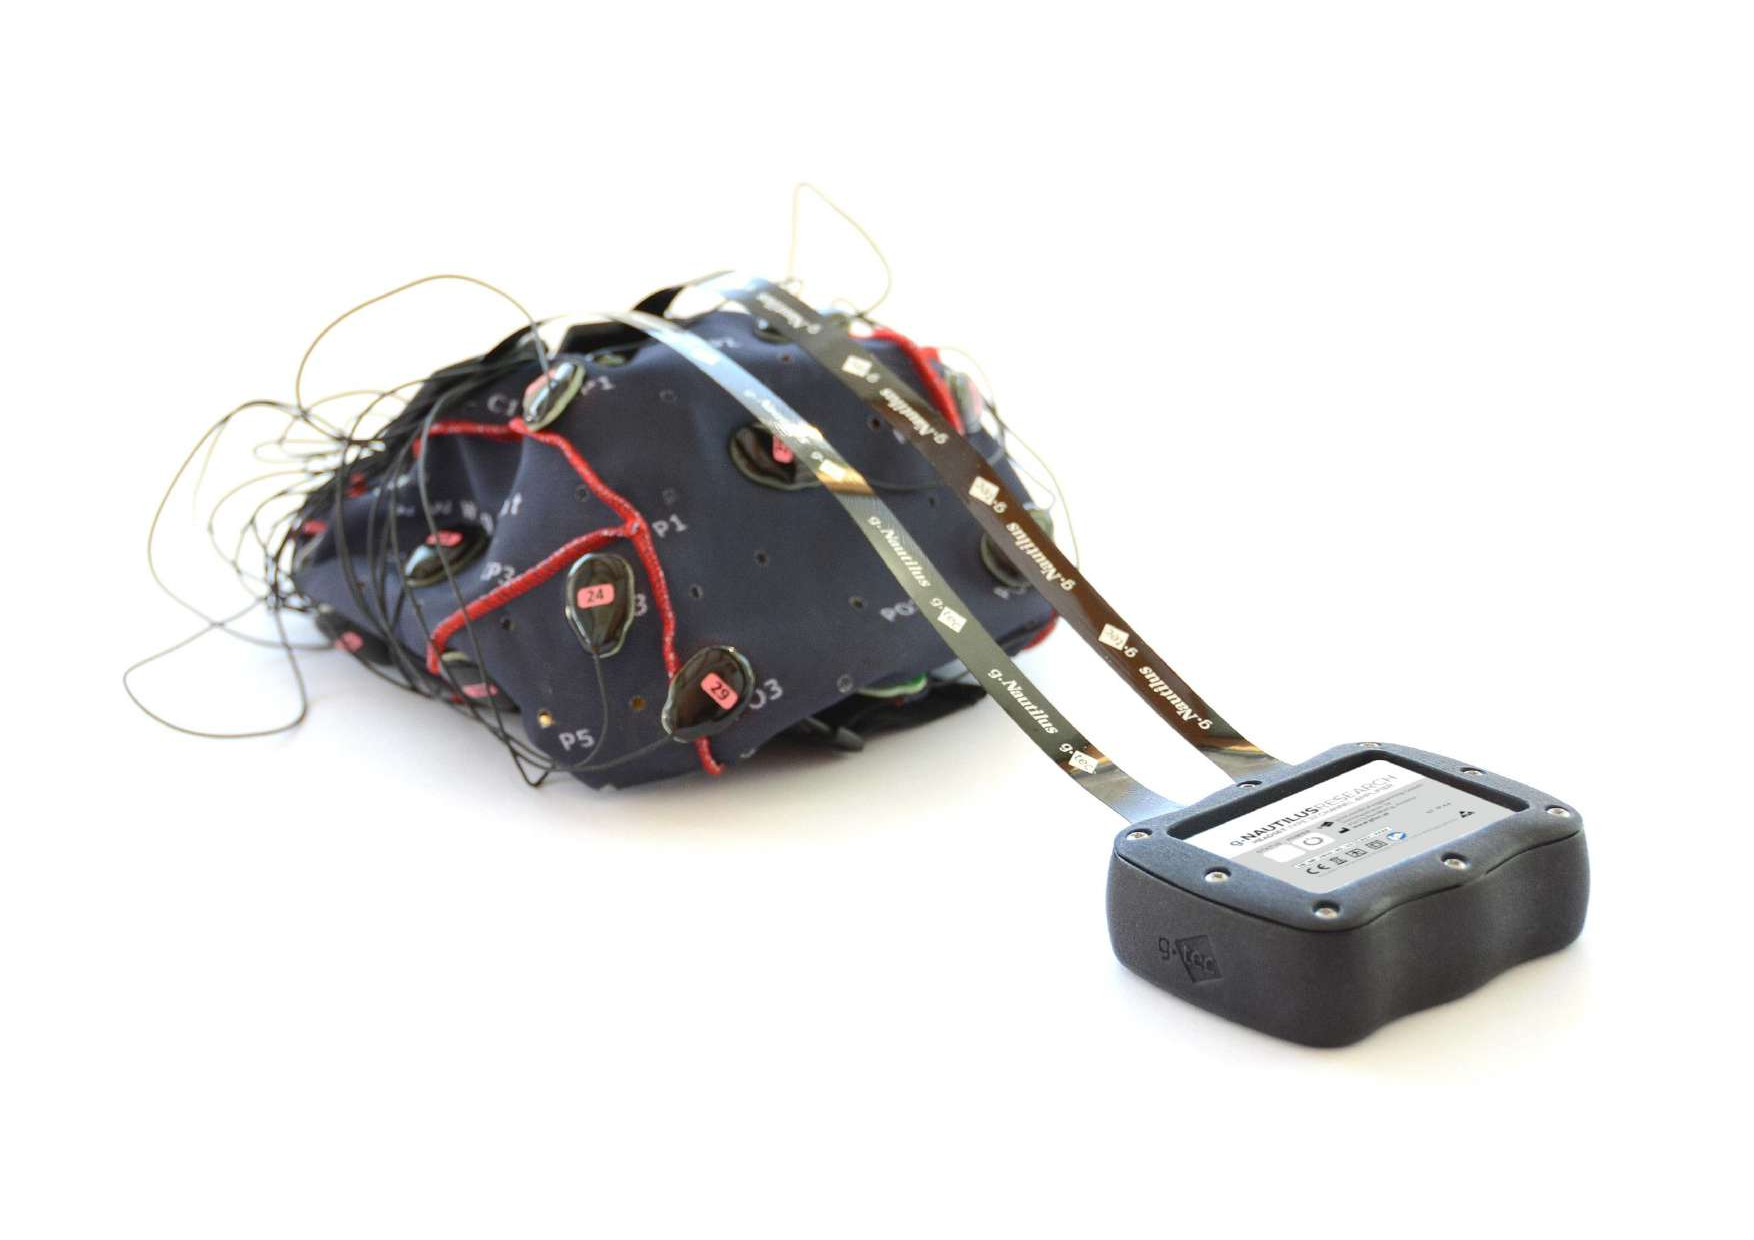
\includegraphics[width=0.4\textwidth]{img/g.Nautilus.pdf}
    \caption{Dispositivo g.Nautilus.}
    \label{fig: g.Nautilus}
\end{figure}

Por lo tanto, el 'g.Nautilus PRO' es una herramienta valiosa para la monitorización cerebral, la investigación y el diagnóstico en entornos médicos y clínicos. Su diseño modular y su capacidad de adaptación lo convierten en una opción versátil para profesionales de la salud y científicos interesados en la actividad cerebral.

\subsection{Uso de BCI para controlar máquinas.}
En 2024, un científico español y su equipo han desarrollado una BCI \cite{ArticuloControlBCI}\footnote{Página del árticulo del desarrollo de una BCI para controlar dispositivos con la mente \cite{ArticuloControlBCI}.}. La posibilidad de controlar dispositivos tecnológicos mediante el pensamiento, ha sido objeto de investigaciones en todo el mundo. Las BCI han demostrado eficacia en el control de exoesqueletos y la traducción de actividad neuronal en palabras. Sin embargo, muchas aproximaciones requieren implantes invasivos.

El investigador español José del R. Millán se ha enfocado en interfaces no invasivas y universales, permitiendo a cualquiera aprender a usarlas. Su equipo recientemente logró que personas sanas controlaran con precisión un coche en un videojuego de carreras utilizando solo la mente, sin mandos físicos. El objetivo de este proyecto es trasladar la BCI al ámbito clínico y mejorar la accesibilidad para personas con discapacidad. Este avance podría allanar el camino para entrenar a pacientes en el manejo de dispositivos de asistencia y neurorrehabilitación controlados por BCI.

El laboratorio del investigador español José del R. Millán se ha dedicado durante más de dos décadas al desarrollo de BCI con el objetivo de ayudar a personas con discapacidades motoras. Estas interfaces permiten a los usuarios controlar dispositivos mediante señales cerebrales, pero su calibración previa suele ser prolongada y específica para cada individuo. La solución propuesta por el equipo de Millán permite una autocalibración más rápida al entender las necesidades y señales cerebrales de cada sujeto. Esto acorta los plazos y facilita el uso del dispositivo sin adaptación previa.

La interfaz no es invasiva y se basa en un gorro rojo con electrodos conectado a un ordenador. Los electrodos captan las señales eléctricas del cerebro, que luego son interpretadas por un descodificador. Los usuarios han logrado controlar un coche en un videojuego,como se muestra en la imagen \ref{fig: ExperimentoBCI}, y un programa de equilibrio de una barra digital, demostrando el éxito de este enfoque en la mejora de la plasticidad neuronal. Este avance podría transformar la vida de personas con discapacidad motora al proporcionarles una forma más eficiente y rápida de interactuar con la tecnología.

\begin{figure}[H]
    \centering
    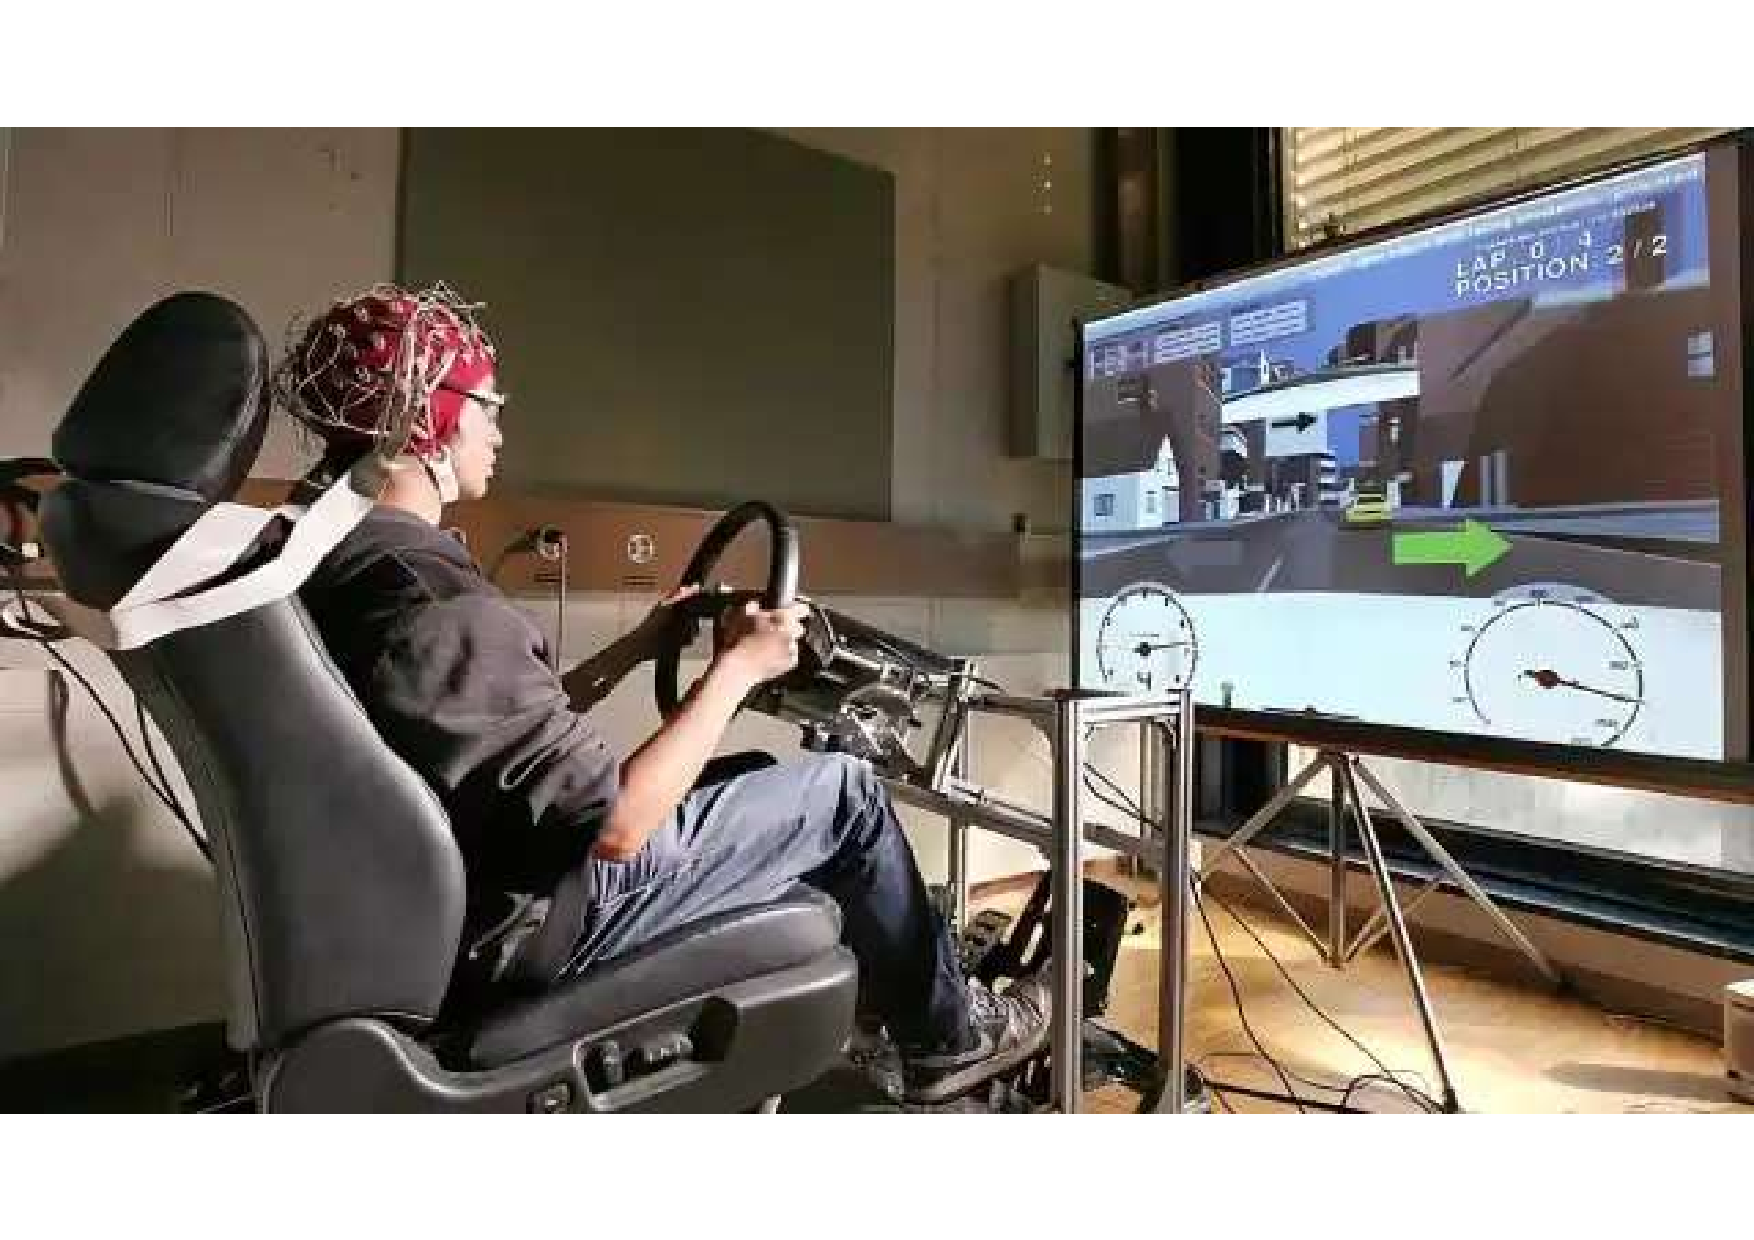
\includegraphics[width=0.6\textwidth]{img/ExperimentoBCI.pdf}
    \caption{Experimento realizado para avanzar en BCI.}
    \label{fig: ExperimentoBCI}
\end{figure}

 El siguiente paso programado por Millán es probar este método con personas que sí sufren algún tipo de discapacidad motora, La posibilidad de producir y distribuir comercialmente un dispositivo de estas características a gran escala aún queda muy lejos, pero esta investigación implica un descubrimiento fundacional, que sienta las bases de futuras innovaciones.

 \subsection{Síntesis del habla y expresiones faciales a partir de señales cerebrales}

 El síndrome de enclaustramiento es un estado neurológico en el que una persona está despierta y consciente, pero presenta cuadriplejía y parálisis de los nervios craneales inferiores. Esto significa que no puede moverse, hablar ni comunicarse, excepto a través de movimientos oculares codificados. Por lo general, se produce después de un accidente cerebrovascular que afecta la protuberancia, interrumpiendo y dañando los centros que controlan la mirada horizontal \cite{SindromeEnclaustramiento}\footnote{Página del NIH con información relativa al síndrome de enclaustramiento \cite{SindromeEnclaustramiento}.}.
 
 Ann Johnson, quien sufrió un derrame cerebral hace casi dos décadas, quedó paralizada y sin capacidad para hablar debido a este síndrome. Sin embargo, con un nuevo implante cerebral basado en inteligencia artificial, ha logrado sintetizar el habla y las expresiones faciales a partir de señales cerebrales, convirtiéndose en la primera paciente en utilizar con éxito esta tecnología innovadora. Los investigadores implantaron electrodos en su cerebro y personalizaron la tecnología para interpretar sus señales cerebrales. Aunque sus músculos no se mueven, su cerebro envía señales que los electrodos descodifican, permitiendo la síntesis del habla y las expresiones faciales mediante un avatar por ordenador.

Antes de este avance, Johnson podía comunicarse a unas 14 palabras por minuto utilizando un antiguo método de mecanografía que respondía a pequeños movimientos de su cabeza. Sin embargo, gracias a la inteligencia artificial, su avatar digital ahora habla a casi 80 palabras por minuto con el nuevo implante. El objetivo de esta tecnología es restablecer una forma de comunicación plena y corporal, que es la manera más natural de interactuar con los demás.

Aunque existen controversias y problemas éticos en el campo de la neurotecnología, avances como este ofrecen posibilidades reales para mejorar la vida humana, siendo un gran ejemplo de cómo la ciencia y la tecnología pueden transformar vidas de maneras inimaginables.
